On the lower-right part of the main window is shown a 3-dimentional representation of the
volume. You can manipulate the volume in different ways:
\begin{itemize}
\item Rotate the volume by moving the mouse while left clicking in the 3D view.
\item Translate the volume by moving the mouse while middle-clicking in the 3D view.
\item Zoom into the volume by moving the mouse up or down while right-clicking in the 3D
  view.
\end{itemize}

\noindent 
\includegraphics[width=1cm]{fullscreen}
You also can display the 3D view in full screen by pressing the ``full screen''
button. When the 3D view is in full screen, you can use the ``snap shot'' button to easily
save a .jpg picture of the current screen.
\ \\

\begin{figure}[htbp]
  \begin{center}
    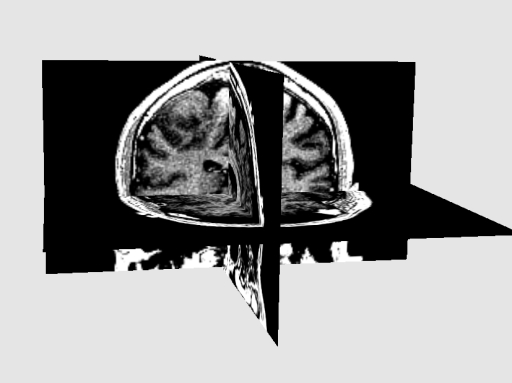
\includegraphics[width=0.45\linewidth]{3Dplanarviews}
    \hspace{0.7cm}
    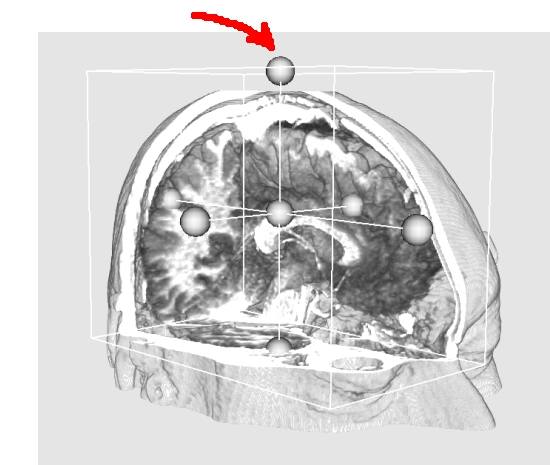
\includegraphics[width=0.45\linewidth]{volumecropped}
  \end{center}
  \caption{ 3D view. You can see on the left a Multi-Planar Reconstruction (MPR) of the image. On
  the right you see a Volume Rendering (VR) of the image, cropped by the cropping box to
  visualize inside the volume. The cropping box can be manipulated by control points (red arrow).
  \label{fig:3Dview}}
\end{figure}

\noindent 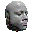
\includegraphics[width=1cm]{volumerendering} You can choose between
displaying an image with Multi-Planar Reconstruction (MPR) (Fig. \ref{fig:3Dview}, right) or with Volume Rendering (VR)
(Fig. \ref{fig:3Dview}, right). When VR mode is chosen, you have the possibility to take
out a part of the volume in order to visualize inside it. This can be done with the ``cropping
box''. Use the control points around the box (red arrow in Fig. \ref{fig:3Dview}, right)
to resize it and crop the volume (left-click on them). The control point in the center of
the box allows you to translate it. When you have finished cropping the volume, you can
make the box disappear by typing ``b'' on your keyboard. The orientation cube and the 3D axes help to recognize the
current orientation of the image, and can be switched on or off with ``i'' keyboard key.
\ \\

\noindent {\large \bf Keyboard and mouse on 3D screen:}
\ \\

\noindent In the 3D view, several optional features are available :\\
- Shift+left-click translates the volume.\\
- Ctrl+left-click rotates the volume around the axis perpendicular to the screen.\\
- Press {\large \bf ``j''} activates ``joystick'' mode (continuous movement mode).\\
- Press {\large \bf ``t''} disables the ``joystick'' mode.\\
- Shift+left-click on the cropping box translates it.\\
- Right-click on the cropping box makes it grow or shrink.\\
- Press {\large \bf ``r''} to center the image.\\
- If you cannot access the cropping box : Press ``b'' to switch it on,
then press the ``center view'' button. If you still don't see it, it may be inside the
volume. Then translate it outside the volume.\\
- If the cropping box doesn't seem to work properly, it might be because it has been flipped over. Use
successively the control points of the box to flip it back to normal. 
